\part{Vertices}
\frame{\partpage}

\begin{frame}{Position}
	\begin{itemize}
		\item Vertices are the basic building blocks of any object
		\pause\item It consists of at least one set of x, y, z coordinates
		\pause\item This represents the position of a vertex in local space
		\pause\item You must provide this x, y, z or the vertex shader will not run
	\end{itemize}
\end{frame}

\begin{frame}{Texture Coordinates}
	\begin{itemize}
		\item We use \textbf{UV coordinates} to refer to points in a texture
		\pause\item $u$ axis is horizontal and ranges from 0 (left) to 1 (right)
		\pause\item $v$ axis is vertical and ranges from 0 (bottom) to 1 (top)
		\pause\item (So really just another name for $xy$ coordinates in texture space)
	\end{itemize}
\end{frame}

\begin{frame}{UV coordinates}
\begin{center}
	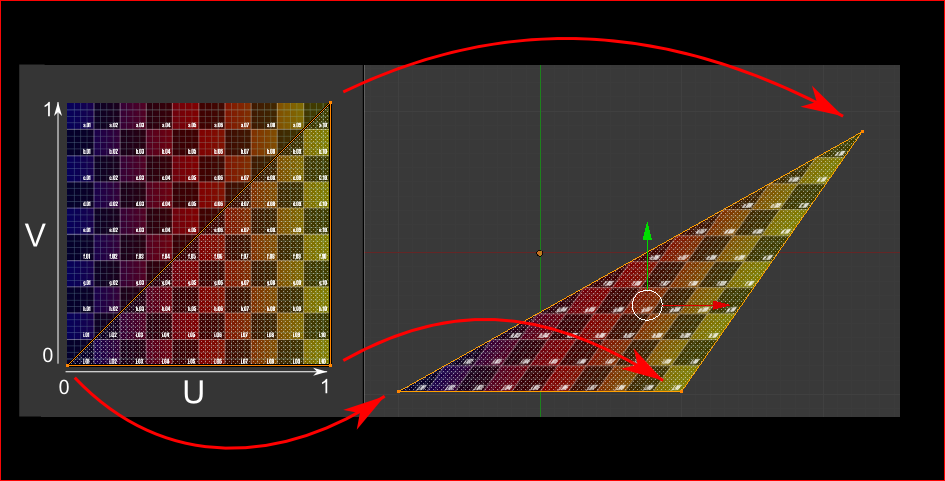
\includegraphics[width=\textwidth]{uv}
\end{center}
\end{frame}

\begin{frame}{Normals}
	\begin{itemize}
		\item Normals are used to specify the direction of a vertex
		\pause\item This is represented as a unit vector (x, y, z)
		\pause\item You can use the dot product of this normal and the light direction, to work out how much light is cast on the surface  
	\end{itemize}
\end{frame}

\begin{frame}{Surface normals}
\begin{columns}
	\pause
	\begin{column}{0.33\textwidth}
		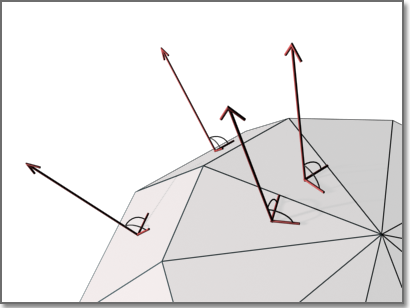
\includegraphics[width=\textwidth]{surface_normal}
	\end{column}
	\begin{column}{0.65\textwidth}
		\begin{itemize}
			\item The \textbf{normal} to a surface is a \textbf{unit vector} that is \textbf{perpendicular} to the surface
			\pause\item If we have two non-parallel vectors that are \textbf{tangent} to the surface, we can use the \textbf{cross product} to find the normal
		\end{itemize}
	\end{column}
\end{columns}
\pause
\begin{columns}
	\begin{column}{0.33\textwidth}
		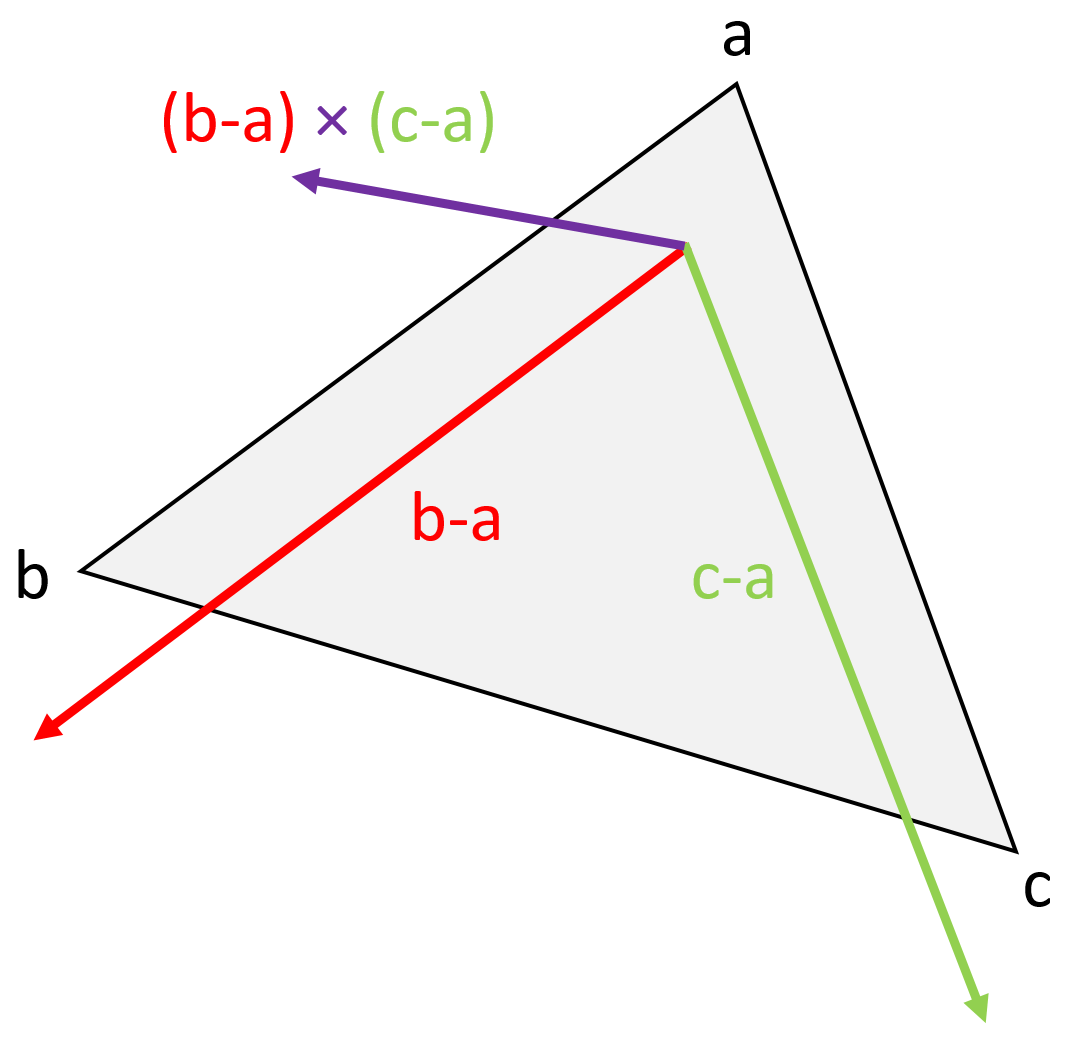
\includegraphics[width=\textwidth]{triangle_normal}
	\end{column}
	\begin{column}{0.65\textwidth}
		\begin{itemize}
			\item For a triangle with vertices $a, b, c$, two such vectors are $b-a$ and $c-a$
			\pause\item So the normal is
			$$ \frac{n}{|n|} \quad \text{where} \quad n = (b-a) \times (c-a) $$
		\end{itemize}
	\end{column}
\end{columns}
\end{frame}

\begin{frame}{Flexible Vertex Format}
	\begin{itemize}
		\item In addition to the above vertex elements there can be
		\begin{itemize}
			\pause \item Vertex Colours - r, g, b, a
			\pause \item Blend Weights - Index of the bone and a float weight
			\pause \item Tangent Normals - x, y, z
		\end{itemize}
		\pause \item There is nothing stopping you encoding any information into these
		\pause \item You could use the vertex colours to hold target positions for animations
	\end{itemize}
\end{frame}

\begin{frame}{Vertex Buffer}
	\begin{itemize}
		\item These vertices are stored in what is know as a Vertex Buffer
		\pause \item In OpenGL and Directx, we fill these up and tell the pipeline what Buffer to use
		\pause \item In UE4 and Unity, these buffers are usually hidden away from us
		\pause \item We typically use higher level classes such as C\# Mesh and UE4 Procedural Mesh to add in our own geometry 
	\end{itemize}
\end{frame}

